\documentclass[12pt]{article}

% Codificación y lenguaje
\usepackage[utf8]{inputenc}
\usepackage[T1]{fontenc}
\usepackage[spanish]{babel}
\usepackage{tikz}
\usetikzlibrary{positioning, arrows.meta}
\usepackage{graphicx} 
\usepackage{tabularx}
\usepackage{hyperref} 

% Márgenes
\usepackage[a4paper, left=2.5cm, right=2.5cm, top=2cm, bottom=2cm]{geometry}

% Gráficos, flotantes y código
\usepackage{graphicx}
\usepackage{float}
\usepackage{listings}
\usepackage{xcolor}
\usepackage{tikz}
\usepackage{url}


% Encabezados y pies de página
\usepackage{fancyhdr}
\pagestyle{fancy}
\fancyhf{}
\lhead{TP Nº2 - Filtrado digital de señales}
\rhead{UNC-Procesamiento digital de señales}
\cfoot{\thepage}

% Estilo para código Matlab
\definecolor{codegreen}{rgb}{0,0.6,0}
\definecolor{codegray}{rgb}{0.5,0.5,0.5}
\definecolor{codepurple}{rgb}{0.58,0,0.82}
\definecolor{backcolour}{rgb}{0.95,0.95,0.92}

\lstdefinestyle{mystyle}{
	language=C,
	backgroundcolor=\color{white},
	basicstyle=\scriptsize\ttfamily,           % Tamaño de fuente reducido con tipografía monoespaciada
	keywordstyle=\color[HTML]{0072BD}\bfseries,
	commentstyle=\color[HTML]{008000}\itshape,
	stringstyle=\color[HTML]{A2142F},
	numberstyle=\tiny\color{gray},             % Números de línea discretos
	numbers=left,
	numbersep=6pt,                             % Separación más generosa para claridad
	frame=single,
	rulecolor=\color{black!50},
	breaklines=true,                           % Cortar líneas largas automáticamente
	breakatwhitespace=false,                   % Cortar incluso sin espacios
	breakautoindent=true,                      % Mantener indentación visual
	tabsize=2,
	showspaces=false,
	showstringspaces=false,
	xleftmargin=1.5em,                         % Margen izquierdo para números
	xrightmargin=0.5em,
	aboveskip=1em,                             % Espacio antes del bloque de código
	belowskip=1em,                             % Espacio después del bloque de código
}

\lstdefinestyle{pythonstyle}{
	language=Python,
	backgroundcolor=\color{white},
	basicstyle=\scriptsize\ttfamily,
	keywordstyle=\color[HTML]{0000FF}\bfseries,
	commentstyle=\color[HTML]{008000}\itshape,
	stringstyle=\color[HTML]{A2142F},
	numberstyle=\tiny\color{gray},
	numbers=left,
	numbersep=6pt,
	frame=single,
	rulecolor=\color{black!50},
	breaklines=true,
	breakatwhitespace=false,
	breakautoindent=true,
	tabsize=4,
	showspaces=false,
	showstringspaces=false,
	xleftmargin=1.5em,
	xrightmargin=0.5em,
	aboveskip=1em,
	belowskip=1em
}


% Título y autores
\title{
	
\includegraphics[width=0.45\textwidth]{unc.png} \\[2cm] % Logo
	\textbf{Trabajo Práctico Nº2: Filtrado digital de señales}
}

\author{
	Profesores: \\ Parlanti Gustavo Fernand (Presidente) \\ Molina German Alcides (Vocal)\\ Rossi Robreto Raul (Vocal)
	\\ \\
	Alumnos:\\ Campos \\ Testa \\ Verstraete 
}

\date{Julio de 2025} % Fecha del trabajo

\begin{document}
	
	\maketitle
	
	\begin{abstract}
		Realizar un programa aplicativo que sea capaz de aplicar un filtro FIR, por muestras, a un buffer de memoria de 512 muestras, que es adquirido con el Laboratorio 1 teniendo en cuenta las frecuencias de muestreo de 8 kHz, 16 kHz, 24 kHz, 40 kHz y 48 kHz.  Con una de las teclas de la placa de evaluación STM32F446RE, se habilitara la aplicación del filtro o se hace bypass del filtro a un buffer de salida distinto del buffer de entrada. De este buffer de salida se enviaran las muestras al DAC de la palca STM32F446RE. Visualizar el resultado utilizando un osciloscopio y comparar los resultados.
		
	\end{abstract}\newpage
	
	\tableofcontents \newpage
	
	\section{Introducción}
	
	El procesamiento digital de señales (DSP) en tiempo real es una disciplina fundamental en aplicaciones embebidas modernas, tales como audio, telecomunicaciones, sensado inteligente,etc. Implementar estos sistemas directamente sobre microcontroladores con recursos limitados impone desafíos tanto computacionales como de diseño. En este contexto, el presente proyecto busca implementar un sistema completo de adquisición, procesamiento y reproducción de señales analógicas en tiempo real, utilizando el microcontrolador STM32F446RE, el cual cuenta con arquitectura ARM Cortex-M4 y soporte para operaciones DSP optimizadas.
	
	Este trabajo continúa el desarrollo iniciado en el primer proyecto. En esta segunda parte, se incorporan capacidades de filtrado digital, trabajando en formato Q15 (punto fijo) para garantizar eficiencia y compatibilidad con la arquitectura.
	
	\subsection{Objetivos del proyecto}
	
	 El sistema conserva la misma arquitectura base del laboratorio anterior —adquisición ADC, procesamiento intermedio, y reproducción DAC—, pero ahora añade la posibilidad de aplicar filtros digitales en tiempo real. Los tipos de filtros implementados incluyen paso bajo (LP), paso alto (HP), pasa banda (BP) y rechazo de banda (BS). El usuario puede seleccionar dinámicamente tanto el tipo de filtro como la frecuencia de muestreo mediante interrupciones externas por GPIO (pulsadores).
	
	\begin{table}[H]
		\centering
		\begin{tabular}{|l|c|c|c|c|}
			\hline
			\textbf{$Tipo$}      & \textbf{$f_{c1}$} & \textbf{$f_{c2}$} & \textbf{$f_{0}$} & \textbf{$BW$} \\
			\hline
			Paso bajo            & 3600 Hz              & --                    & --             & --          \\
			\hline
			Paso alto            & --                   & 35 Hz                 & --             & --          \\
			\hline
			Pasa banda           & 35 Hz                & 3500 Hz               & --             & --          \\
			\hline
			Rechazo de banda     & --                   & --                    & 50 Hz          & 15 Hz       \\
			\hline
		\end{tabular}
		\caption{Parámetros de diseño para cada tipo de filtro}
		\label{tabla:filtros}
	\end{table}
	
	Respecto a los requerimientos de atenuación en la banda de rechazo de los filtros, debe estar en el orden de los 25 a 30 dB.
	
	\subsection{Aspectos a tener en cuenta}
	
	\begin{itemize}
		\item Para lograr un sistema de procesamiento en tiempo real, se mantienen las mismas técnicas que el laboratorio anterior enfocadas en reducir la latencia del sistema. En primer lugar, se utiliza un esquema de doble buffer mediante DMA para la transferencia eficiente de datos entre el ADC/DAC y la memoria RAM, evitando cuellos de botella en la ejecución. La arquitectura ARM Cortex-M4 de la STM32F446RE permite aprovechar la unidad de punto fijo con saturación (\texttt{DSP extension}) y el contador de ciclos DWT, lo cual resulta clave para medir el rendimiento del sistema.
		
		\item Otro aspecto crucial es el correcto escalado y normalización de los datos. La señal adquirida del ADC de 12 bits es convertida a formato Q15 para ser procesada por la biblioteca \texttt{CMSIS-DSP}, y luego reconvertida al rango del DAC, que también es de 12 bits.\newpage
		
		\item Se debe contemplar que el sistema debe operar a distintas frecuencias de muestreo (8 kHz, 16 kHz, 24 kHz, 40 kHz y 48 kHz), lo cual exige una correcta reconfiguración del temporizador de disparo y la selección de coeficientes adecuados para cada filtro y frecuencia (el cambio de frecuencia de muestreo cambia los coeficientes, por mas que el filtro sea el mismo tipo). El sistema cuenta también con retroalimentación visual mediante LED RGB para indicar el estado actual del muestreo, y contempla un modo de parada segura (modo 5) para evitar errores o conflictos cuando se reconfigura dinámicamente el sistema.
		
		\item Por ultimo el calculo y diseño de los filtros debe apegarse a los requerimientos mencionados en el cuadro anterior. Como se explica posteriormente en la sección 4, no es posible su implementación con los filtros de tipo FIR, por lo que se opto por implementarlos con filtros IIR, estos tipos de filtros son capaces de cumplir con las especificaciones de frecuencia de corte y atenuación en las bandas, a expensas de perder linealidad en la fase y poder tener problemas de estabilidad.
	\end{itemize}
	
	\section{Marco teórico}
	
	El filtrado digital es una operación fundamental dentro del procesamiento digital de señales (DSP), utilizada para modificar el contenido espectral de una señal, suprimiendo componentes no deseados o destacando frecuencias de interés. En sistemas embebidos de tiempo real, como los basados en microcontroladores ARM Cortex-M, es indispensable implementar filtros eficientes que cumplan con los requerimientos funcionales sin comprometer el rendimiento del sistema.
	
	\subsection{Conceptos fundamentales del filtrado digital}
	
	Un filtro digital es un sistema que transforma una señal de entrada $x[n]$ en una señal de salida $y[n]$, aplicando una operación matemática determinada. Los filtros pueden clasificarse en diversas categorías según su comportamiento en frecuencia (paso bajo, paso alto, pasa banda, rechazo de banda) y según su estructura (FIR o IIR). Los objetivos típicos del filtrado son:
	
	\begin{itemize}
		\item Atenuar ruido o interferencias.
		\item Extraer información útil dentro de una banda específica.
		\item Suavizar o eliminar fluctuaciones rápidas en la señal.
		\item Adaptar el contenido espectral de la señal para análisis posterior.
	\end{itemize}
	
	\subsection{Filtros FIR}
	
	Filtros FIR (Finite Impulse Response): Son filtros cuya respuesta al impulso es finita, ya que dependen únicamente de muestras pasadas de la señal de entrada. Su estructura general es:
	
	\begin{equation}
		y[n] = \sum_{k=0}^{N} b_k x[n-k]
	\end{equation}\newpage
	
	Tienen las siguientes características:
	\begin{itemize}
		\item Siempre estables.
		\item Fase lineal.
		\item Requieren más coeficientes para lograr altas pendientes de atenuación.
	\end{itemize}
	
	\subsubsection{Diseño de filtros FIR y el uso de ventanas}
	El diseño de filtros FIR (Finite Impulse Response) parte, generalmente, de una respuesta ideal en frecuencia. Por ejemplo, un filtro paso bajo ideal tendría una transición perfectamente abrupta entre la banda pasante y la banda atenuada, lo cual implica una respuesta al impulso infinita. Como esto no es realizable en sistemas discretos, se realiza una truncación temporal de esa respuesta, lo cual equivale a multiplicarla por una ventana rectangular en el dominio temporal.Sin embargo, esta truncación introduce efectos no deseados en la respuesta en frecuencia, principalmente el llamado fenómeno de Gibbs. \\ 
	
	Fenómeno de Gibbs: Es una oscilación persistente (rizado o \textit{ripple}) que aparece cerca de las discontinuidades en la respuesta en frecuencia del filtro debido a la truncación abrupta de la respuesta al impulso, este efecto provoca:
	
	\begin{itemize}
		\item Rizado en la banda pasante y/o banda de detención.
		\item Ensanchamiento de la zona de transición.
		\item Picos de sobrepaso que no desaparecen al aumentar el número de coeficientes (aunque se concentran en un área más estrecha).
	\end{itemize}
	
	Para mitigar el fenómeno de Gibbs y mejorar el comportamiento espectral del filtro, se utilizan funciones ventana, que consisten en aplicar un suavizado gradual a los extremos de la respuesta al impulso truncada. Este procedimiento reduce el rizado a costa de un ensanchamiento adicional en la zona de transición, representando un compromiso entre precisión en frecuencia y suavidad espectral, las ventanas mas comunes son:
	
	\begin{itemize}
		\item \textbf{Hamming:} Buena atenuación lateral con transiciones moderadas.
		\item \textbf{Hann:} Similar a Hamming pero con menor atenuación lateral.
		\item \textbf{Blackman:} Alta atenuación lateral, pero con una transición más ancha.
		\item \textbf{Rectangular:} Equivale a no aplicar ventana. Genera el mayor rizado (fenómeno de Gibbs más pronunciado).
	\end{itemize}
	
	La elección de la ventana depende de las prioridades del diseño: una mejor atenuación fuera de banda o una transición más angosta. Es importante destacar que este método de diseño con ventanas es exclusivo de filtros FIR, ya que los filtros IIR se diseñan a partir de aproximaciones analíticas (como Butterworth o Chebyshev) y no requieren truncación ni uso de ventanas.
	
	\begin{table}[H]
		\centering
		\begin{tabularx}{\textwidth}{|l|c|c|X|}
			\hline
			\textbf{Ventana} & \textbf{Ancho de banda} & \textbf{Atenuación lateral} & \textbf{Uso típico} \\
			\hline
			Rectangular & Estrecho (mejor) & $\approx$ -13 dB & Alta resolución, pero máximo ripple (Gibbs marcado) \\
			\hline
			Hamming     & Moderado          & $\approx$ -43 dB & Buen compromiso entre transición y atenuación \\
			\hline
			Hann        & Moderado          & $\approx$ -31 dB & Menor ripple que Hamming, pero peor resolución \\
			\hline
			Blackman    & Ancho (peor)      & $\approx$ -58 dB & Muy buena supresión lateral, transición más ancha \\
			\hline
			Kaiser ($\beta$ variable) & Ajustable & Ajustable & Permite ajustar entre resolución y atenuación según $\beta$ \\
			\hline
		\end{tabularx}
		\caption{Características principales de funciones ventana comunes en diseño FIR}
		\label{tabla:ventanas}
	\end{table}
	
	
	\subsection{Filtros IIR}
	Filtros IIR (Infinite Impulse Response): se caracterizan por poseer una respuesta al impulso de duración infinita. Esto se debe a que incluyen términos de retroalimentación, es decir, la salida actual del sistema depende tanto de entradas presentes y pasadas como de salidas pasadas. Su expresión general en forma de ecuación en diferencias se escribe como:
	
	\begin{equation}
		y[n] = \sum_{k=0}^{M} b_k x[n-k] - \sum_{k=1}^{N} a_k y[n-k]
	\end{equation}
	
	Características principales:
	\begin{itemize}
		\item Requieren menos coeficientes que un FIR para lograr especificaciones similares.
		\item Son más eficientes computacionalmente.
		\item Pueden presentar problemas de estabilidad si no se diseñan correctamente.
	\end{itemize}
	
	\subsubsection{Filtros biquad y cascada de secciones}
	En la implementación práctica de filtros IIR, especialmente en sistemas digitales con aritmética de punto fijo como los microcontroladores, es habitual descomponer el filtro en secciones de segundo orden denominadas biquads. Cada biquad corresponde a un filtro de segundo orden cuya estructura es más robusta frente a errores numéricos. La ecuación que describe una sección biquad es:
	
	\begin{equation}
		y[n] = b_0 x[n] + b_1 x[n-1] + b_2 x[n-2] - a_1 y[n-1] - a_2 y[n-2]
	\end{equation}
	
	Para filtros de orden superior, varias de estas secciones se encadenan en forma de cascada. Esta estrategia permite controlar mejor la ganancia interna del sistema, aplicar escalado para prevenir desbordamientos (post-shift), y facilitar el ajuste de parámetros individuales. Además, mejora la estabilidad numérica general del filtro, lo que es especialmente importante en contextos de baja resolución, como en procesadores digitales de señales con punto fijo.\newpage
	
	A diferencia de los filtros FIR, que son siempre estables si sus coeficientes son finitos, los filtros IIR pueden volverse inestables debido a la presencia de realimentación. La estabilidad de un filtro IIR depende de la ubicación de los polos de su función de transferencia en el plano-z; para que sea estable, todos los polos deben estar dentro del círculo unitario. Esto implica que el diseño de filtros IIR requiere un mayor cuidado en la selección de coeficientes, especialmente en implementaciones con precisión limitada, como las de punto fijo. En contraste, los filtros FIR no presentan este tipo de limitaciones estructurales, lo que los hace más robustos desde el punto de vista de la estabilidad, aunque a costa de una mayor complejidad computacional para alcanzar el mismo rendimiento en frecuencia.
	
	\subsection{Implementación con la biblioteca CMSIS-DSP}
	
	La biblioteca \texttt{CMSIS-DSP}, desarrollada por ARM, proporciona un conjunto de funciones optimizadas para realizar procesamiento digital de señales en microcontroladores con núcleo Cortex-M. Su diseño está pensado para maximizar el rendimiento utilizando instrucciones SIMD cuando están disponibles, y ofrece soporte tanto para punto fijo (\texttt{Q15}) como para punto flotante (\texttt{float32}). Entre sus herramientas más destacadas se encuentran funciones específicas para el diseño y ejecución de filtros FIR e IIR.
	
	Para implementar un filtro IIR en cascada de secciones biquad utilizando CMSIS-DSP en formato \texttt{Q15}, es fundamental seguir una secuencia precisa de pasos. En primer lugar, se deben calcular los coeficientes del filtro, los cuales deben estar organizados en bloques de cinco valores por sección biquad: tres coeficientes para la parte directa (\texttt{b0}, \texttt{b1}, \texttt{b2}) y dos para la parte recursiva (\texttt{a1}, \texttt{a2}). Estos coeficientes deben ser previamente escalados y convertidos al formato \texttt{Q15}, lo cual puede hacerse con herramientas como MATLAB, Python (SciPy) o incluso manualmente si el diseño es simple. El siguiente paso consiste en preparar la estructura de datos \texttt{arm\_biquad\_casd\_df1\_inst\_q15}, la cual describe el filtro. Esta estructura debe contener el número de etapas, un puntero al arreglo de coeficientes, un puntero al buffer de estado (de longitud \texttt{4 × numStages}) y el parámetro \texttt{postShift}, que ajusta el escalado de salida para prevenir saturación en aritmética de punto fijo.Con estos datos definidos, se debe llamar a la función \texttt{arm\_biquad\_cascade\_df1\_init\_q15}, que inicializa la estructura asociando los arreglos y parámetros con los campos internos del filtro. Este paso es obligatorio antes de aplicar el procesamiento.
	
	Una vez inicializado, el filtro puede aplicarse sobre un bloque de muestras utilizando la función \texttt{arm\_biquad\_cascade\_df1\_q15}, la cual toma como argumentos la estructura, un puntero al arreglo de entrada, otro al de salida, y la cantidad de muestras. Esta función recorre cada muestra, aplicando todas las etapas en cascada y actualizando automáticamente el estado interno.
	
	Respetar esta secuencia —definición de coeficientes, asignación del buffer de estado, configuración de parámetros, inicialización y luego procesamiento— es fundamental para que el filtro funcione correctamente y se eviten errores comunes como desbordamientos o accesos inválidos a memoria.
	
	Toda la documentación oficial puede consultarse en el sitio web de ARM:\newline \href{https://www.keil.com/pack/doc/CMSIS/DSP/html/index.html}{https://www.keil.com/pack/doc/CMSIS/DSP/html/index.html}.
	
    \newpage
	
	\section{Placa de Desarrollo y Herramientas Utilizadas}
	El proyecto fue desarrollado sobre la placa STM32 Nucleo-F446RE, basada en el microcontrolador STM32F446RE, perteneciente a la familia STM32F4 de STMicroelectronics. Esta plataforma integra una arquitectura avanzada ARM Cortex-M4, periféricos orientados a procesamiento de señales, y herramientas de desarrollo que permiten implementar sistemas en tiempo real de forma eficiente.
	
	\begin{figure}[h!]
		\centering
		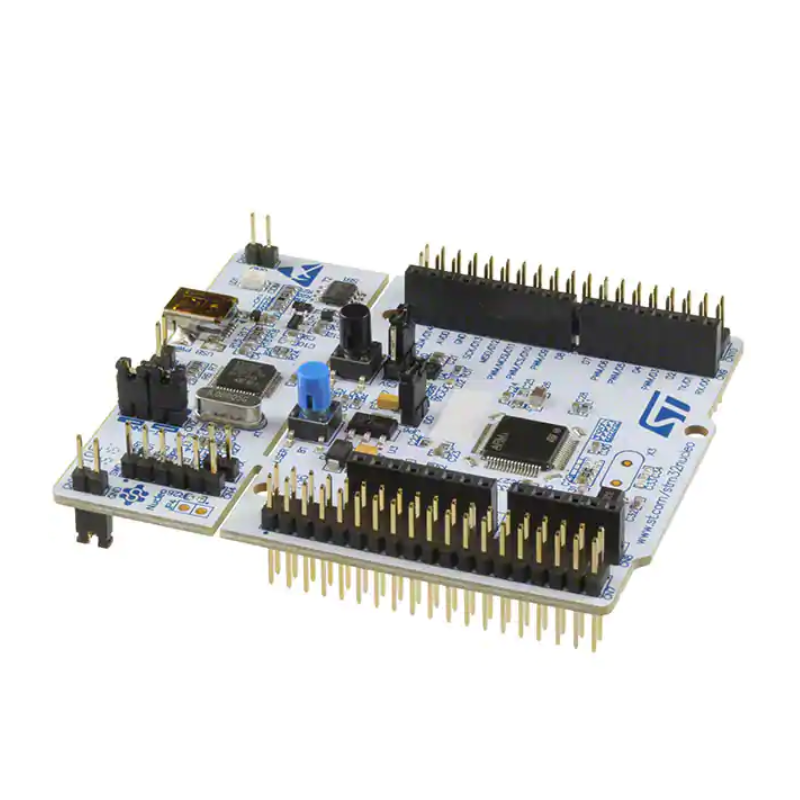
\includegraphics[width=0.7\linewidth]{placa}
		\caption[Placa de desarrollo]{Placa de desarrollo}
		\label{fig:placa}
	\end{figure}
	
	\subsection{Microcontrolador STM32F446RE}
	El STM32F446RE es un microcontrolador de 32 bits basado en el núcleo ARM Cortex-M4, optimizado para procesamiento digital con soporte de instrucciones DSP y unidad de punto flotante opcional (FPU simple precisión). Sus principales características relevantes al proyecto son:
	
	\begin{itemize}
		\item Frecuencia de operación: hasta 180MHz
		
		\item Memoria Flash: 512KB
		
		\item RAM: 128KB
		
		\item Tensión de operación: 1.8V a 3.6V
		
		\item Paquete: LQFP64 (compatible con la Nucleo-F446RE)
	\end{itemize}
	
		\subsection{Periféricos clave utilizados}
	\subsubsection{ADC (Analog-to-Digital Converter)}
	El STM32F446RE cuenta con 3 ADCs independientes (ADC1, ADC2 y ADC3), cada uno de 12 bits de resolución y con capacidad de hasta 2.4 MSPS (mega muestras por segundo) en modo intercalado. Para este proyecto se utiliza el ADC1 en modo regular y con DMA activado. Sus características técnicas relevantes incluyen:
	
	\begin{itemize}
		\item Resolución seleccionable: 6, 8, 10 o 12 bits (se usa 12 bits para mayor precisión).
		
		\item Tasa de muestreo máxima (single conversion): hasta 2.4 MSPS.
		
		\item Rango de entrada: 0V a VREF (típicamente 3.3V).
		
		\item Tiempo de muestreo configurable: desde 3 hasta 480 ciclos de ADC.
		
		\item Trigger externo: el inicio de la conversión puede ser disparado por un temporizador, lo cual permite muestrear a frecuencias precisas.
		
		\item Modo DMA: transferencia automática de los resultados a un buffer en memoria (sin intervención del CPU).
		
		\item Modo continuo + DMA circular: permite muestreo ininterrumpido con mínimo overhead.
	\end{itemize}
	
	\subsubsection{DAC (Digital-to-Analog Converter)}
	El STM32F446RE incluye 2 canales DAC (DAC1 y DAC2), ambos de 12 bits, con capacidad de salida en modo bufferizado (con baja impedancia) o sin buffer (alta velocidad). Se utiliza DAC1 en este proyecto para convertir las muestras digitales de salida nuevamente en una señal analógica. Características clave:
	
	\begin{itemize}
		\item Resolución de conversión: 12, 10 u 8 bits.
		
		\item Velocidad típica: hasta 1 MSPS (modo sin buffer).
		
		\item Modo bufferizado: reduce el ruido, ideal para salidas de audio.
		
		\item Trigger externo: puede sincronizarse con un temporizador (por ejemplo TIM6/TRGO).
		
		\item Soporte DMA: se permite la alimentación directa de datos desde memoria al DAC sin CPU.
		
		\item Salidas disponibles: a través de pines analógicos dedicados (por ejemplo, PA4 para DAC1).
	\end{itemize}
	
	\subsubsection{DMA (Direct Memory Access)}
	El controlador DMA2 es utilizado para las transferencias entre ADC/DAC y RAM. El STM32F446RE cuenta con dos controladores DMA (DMA1 y DMA2), con un total de 16 canales (streams) y soporte para múltiples periféricos. Características específicas:
	
	\begin{itemize}
		\item Transferencia en background, sin intervención del CPU.
		
		\item Modo circular: ideal para buffers cíclicos o doble buffering.
		
		\item Prioridad programable por canal.
		
		\item Transferencia por palabras (16 bits en Q15).
		
		\item Eventos por mitad de buffer y buffer completo: permite usar doble buffer sincronizado.
	\end{itemize}
	
	\subsubsection{TIM (Timers)}
	El STM32F446RE cuenta con 14 temporizadores (4 avanzados, 2 básicos, 8 generales), todos con configuraciones de prescaler, auto-reload y posibilidad de generar eventos de actualización. Se utilizan para generar señales periódicas que actúan como trigger de muestreo. Características clave:
	\begin{itemize}
		\item TIM2-TIM5: de 32 bits, con amplio rango de conteo (útiles para precisión en frecuencias bajas).
		
		\item Configuración de frecuencia: vía Prescaler y ARR (Auto-Reload Register).
		
		\item Trigger de ADC/DAC: mediante señal TRGO (Trigger Output).
		
		\item Modo master-slave: permite sincronización entre periféricos.
	\end{itemize}
	
	\subsubsection{GPIO – General Purpose Input/Output}
	Los pines GPIO permiten la interacción con el usuario mediante botones (teclas) y LEDs. Se utilizan:
	
	\begin{itemize}
		\item Velocidad de salida seleccionable: Low, Medium, Fast, High.
		
		\item Pull-up/Pull-down configurables.
		
		\item Interrupciones por flanco ascendente, descendente o ambos.
	\end{itemize}
	
	\subsubsection{Herramientas de desarrollo}
	Para la implementación del proyecto se utilizaron las siguientes herramientas:
	
	\begin{itemize}
		\item STM32CubeIDE: entorno de desarrollo oficial de STMicroelectronics, basado en Eclipse, que permite configurar periféricos gráficamente, generar código y compilar con GCC.
		
		\item STM32CubeMX: herramienta para la configuración inicial de pines, relojes, periféricos y generación de código base.
		
		\item CMSIS y CMSIS-DSP: bibliotecas proporcionadas por ARM para facilitar el uso de instrucciones de bajo nivel y rutinas DSP optimizadas en punto fijo.
		
		\item GDB y ST-Link: utilizados para depuración, profiling y medición de tiempos mediante DWT->CYCCNT.
	\end{itemize}\newpage
	
	\begin{figure}[h!]
		\centering
		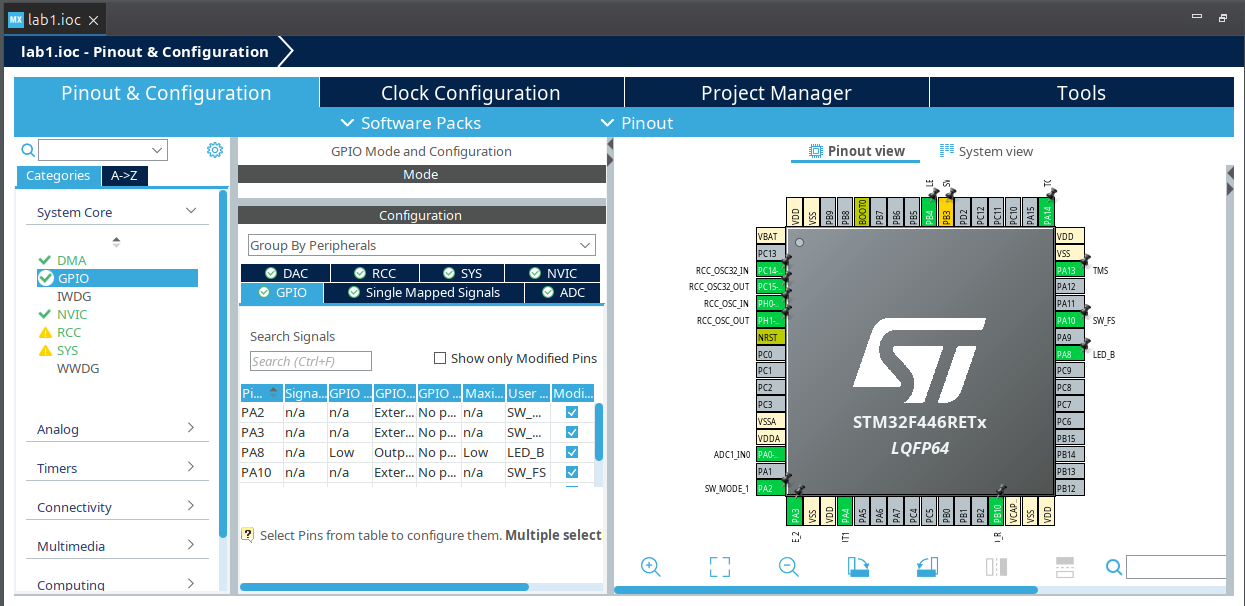
\includegraphics[width=1\linewidth]{IDE}
		\caption[Entorno de desarrollo STM32CUBE IDE]{Entorno de desarrollo STM32CUBE IDE}
		\label{fig:ide}
	\end{figure}
	
	\section{Calculo y diseño de filtros}
	El siguiente script en Python permite diseñar, visualizar y exportar filtros digitales IIR en formato compatible con la biblioteca CMSIS-DSP, especialmente para su uso en microcontroladores que trabajan con aritmética en punto fijo (Q15). Se definen varios tipos de filtros (pasa bajos, pasa altos, pasa banda y notch) y se evalúan sus respuestas en frecuencia para distintas frecuencias de muestreo. Cada filtro se diseña utilizando funciones de la biblioteca SciPy (\texttt{butter} para filtros clásicos y \texttt{iirnotch} para el notch), y luego se convierte a la forma de secciones en cascada (\texttt{tf2sos}) para garantizar estabilidad numérica. A partir de las secciones obtenidas, se calcula un valor de \texttt{postShift} sugerido que permite escalar correctamente los coeficientes al formato Q15 sin riesgo de saturación. Los coeficientes se imprimen en formato C, listos para ser copiados directamente en un proyecto basado en CMSIS-DSP, junto con los buffers de estado necesarios para cada configuración. Además, el script genera diagramas de Bode que permiten visualizar y comparar gráficamente el comportamiento en frecuencia de los filtros para distintas frecuencias de muestreo.
	
	\begin{lstlisting}[style=pythonstyle]
		import numpy as np
		import matplotlib.pyplot as plt
		from scipy.signal import butter, iirnotch, tf2sos, sosfreqz
		# === Parametros generales ===
		fs_list = [8000, 16000, 24000, 40000, 48000]
		orden = 2
		# === Especificaciones por tipo ===
		filtros = {
			"low":  {"type": "lowpass",  "params": {"fc": 3600}},
			"high": {"type": "highpass", "params": {"fc": 35}},
			"band": {"type": "bandpass", "params": {"fc1": 35, "fc2": 3500}},
			"band_stop": {"type": "band_stop",   "params": {"f0": 50, "bw": 30}},  # Q = f0 / bw
		}
		# === Conversion a Q15 ===
		def to_q15(x):
		return max(min(int(round(x * 32767)), 32767), -32768)
		# === Loop por tipo de filtro y frecuencia de muestreo ===
		for filt_name, spec in filtros.items():
		plt.figure(figsize=(8, 5))
		for fs in fs_list:
		nyq = fs / 2
		tipo = spec["type"]
		params = spec["params"]
		# ==== Diseno del filtro ====
		if tipo == "lowpass":
		Wn = params["fc"] / nyq
		b, a = butter(orden, Wn, btype='low')
		elif tipo == "highpass":
		Wn = params["fc"] / nyq
		b, a = butter(orden, Wn, btype='high')
		elif tipo == "bandpass":
		fc1 = params["fc1"] / nyq
		fc2 = params["fc2"] / nyq
		b, a = butter(orden, [fc1, fc2], btype='band')
		elif tipo == "band_stop":
		f0 = params["f0"]
		Q = f0 / params["bw"]
		w0 = f0 / nyq
		b, a = iirnotch(w0=w0, Q=Q)
		else:
		continue
		sos = tf2sos(b, a)
		var_name = f"{filt_name}_{fs // 1000}k"
		# ==== Calcular postShift sugerido ====
		# Maximo coeficiente absoluto en punto flotante (solo numerador y denominador de cada seccion)
		max_coef = 0.0
		for sec in sos:
		b0, b1, b2, a0, a1, a2 = sec
		max_sec = max(abs(b0), abs(b1), abs(b2), abs(a1), abs(a2))
		if max_sec > max_coef:
		max_coef = max_sec
		# Escalado para evitar overflow en Q15 (coef entre -1 y 1 * 32767)
		post_shift = max(0, int(np.floor(np.log2(32767 / max_coef))))
		# ==== Generacion de coeficientes Q15 ====
		print(f"\n// ===== {tipo.upper()} Filter =====")
		print(f"// fs = {fs} Hz")
		print(f"// CMSIS-DSP format: {{b0, b1, b2, -a1, -a2}} in Q15")
		print(f"// Suggested postShift: {post_shift}")
		print(f"#define stage_{var_name} {len(sos)}")
		print(f"q15_t {var_name}[5 * stage_{var_name}] = {{")
				for sec in sos:
				b0, b1, b2, a0, a1, a2 = sec
				assert np.isclose(a0, 1.0, atol=1e-4), "a0 must be 1.0 for CMSIS-DSP"
				b_q15 = [to_q15(c) for c in [b0, b1, b2]]
				a_q15 = [to_q15(-a1), to_q15(-a2)]
				line = "    " + ", ".join(f"{v:6d}" for v in (b_q15 + a_q15)) + ","
				print(line)
				print("};")
			print(f"q15_t {var_name}_status[4 * stage_{var_name}] = {{ 0 }};\n")
			# ==== Diagrama de Bode ====
			w, h = sosfreqz(sos, worN=1024, fs=fs)
			plt.semilogx(w, 20 * np.log10(np.maximum(np.abs(h), 1e-5)), label=f"{fs//1000}kHz")
			
			# === Grafico por tipo de filtro ===
			plt.title(f"Bode Plot - {tipo.title()} Filter")
			plt.xlabel("Frequency [Hz]")
			plt.ylabel("Magnitude [dB]")
			plt.grid(which='both', linestyle='--', linewidth=0.5)
			plt.axvline(params.get("fc", params.get("f0", params.get("fc1"))), color='red', linestyle=':', label="Reference Frequency")
			if tipo == "bandpass":
			plt.axvline(params["fc2"], color='red', linestyle=':')
			elif tipo == "band_stop":
			plt.axvline(params["f0"], color='red', linestyle=':')
			plt.legend()
			plt.tight_layout()
			plt.show()
	\end{lstlisting}
	
	\begin{figure}
		\centering
		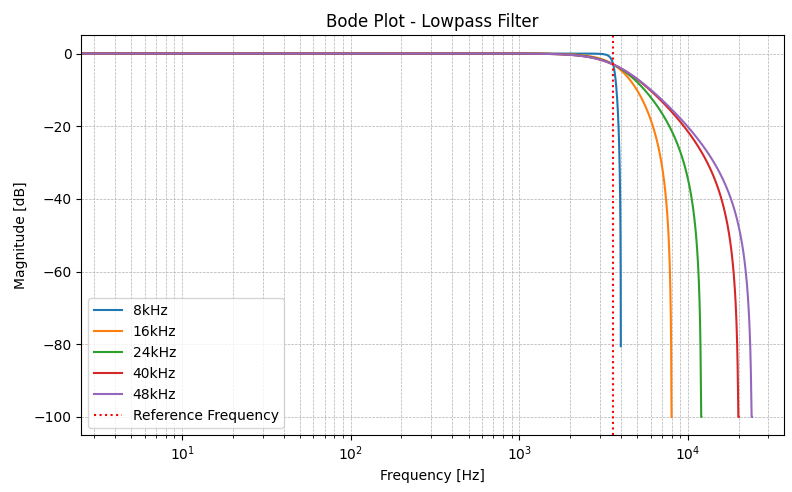
\includegraphics[width=1\linewidth]{pasa_bajo}
		\caption[Diagrama de bode: Filtros pasa bajo]{Diagrama de bode: Filtros pasa bajo}
		\label{fig:pasabajo}
	\end{figure}
	
	\begin{figure}
		\centering
		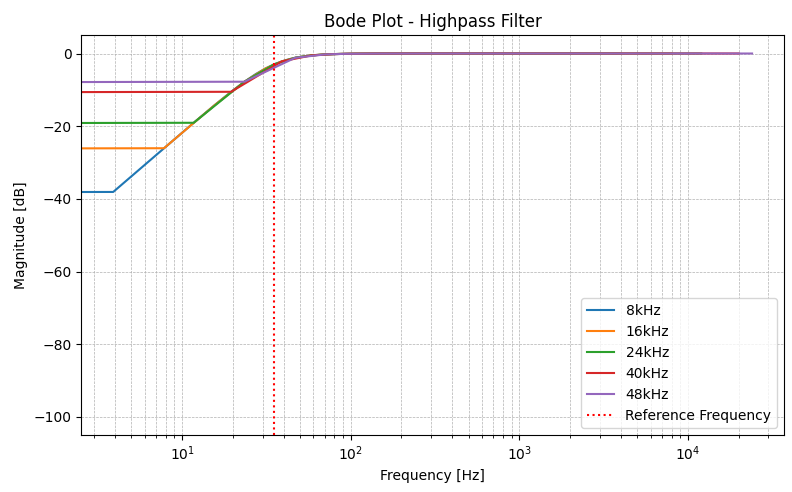
\includegraphics[width=1\linewidth]{pasa_alto}
		\caption[Diagrama de bode: Filtros pasa alto]{Diagrama de bode: Filtros pasa alto}
		\label{fig:pasaalto}
	\end{figure}\newpage
	
	\begin{figure}
		\centering
		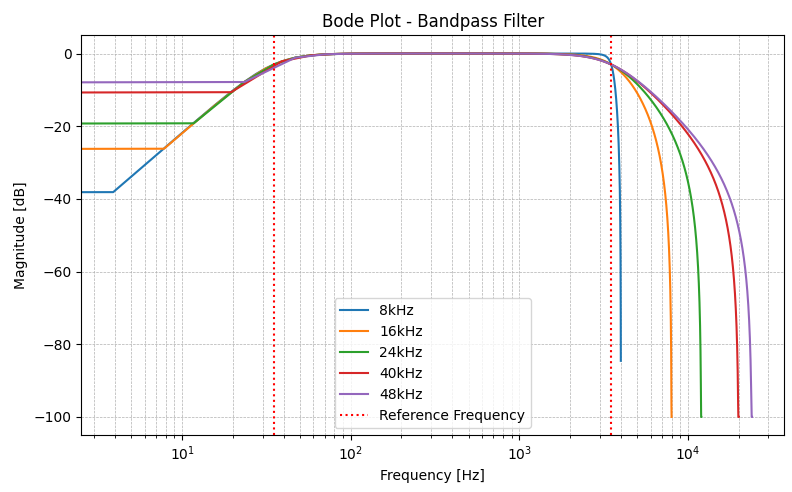
\includegraphics[width=1\linewidth]{pasa_banda}
		\caption[Diagrama de bode: Filtros pasa banda]{Diagrama de bode: Filtro pasa banda}
		\label{fig:pasabanda}
	\end{figure}
	
	\begin{figure}[h!]
		\centering
		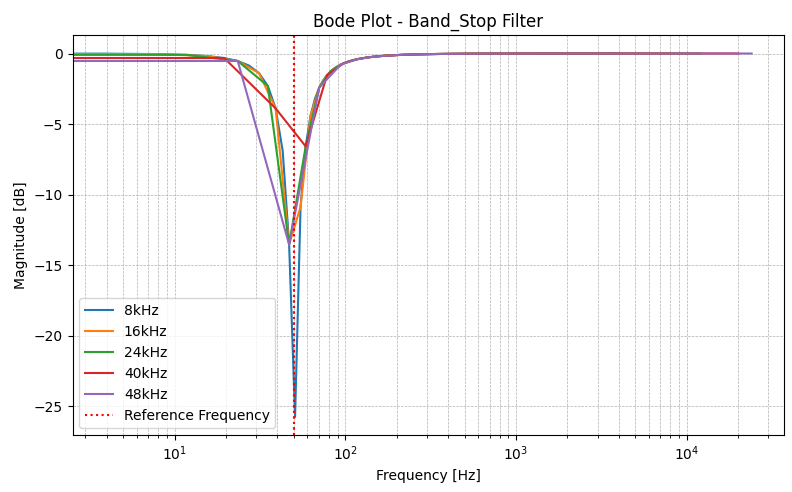
\includegraphics[width=1\linewidth]{rechaza_banda}
		\caption[Diagrama de bode: Filtros rechaza banda]{Diagrama de bode: Filtros rechaza banda}
		\label{fig:rechazabanda}
	\end{figure}

	
	\section{Diseño del programa}

	El sistema implementado permite procesar una señal en tiempo real utilizando el microcontrolador STM32F446RE. La estructura general es similar a la utilizada en el Trabajo Práctico Nº1, incorporando en este caso una etapa de filtrado digital mediante filtros FIR implementados con la biblioteca CMSIS-DSP.

	El funcionamiento del sistema comienza con la inicialización de los periféricos necesarios: GPIO, DMA, ADC, DAC y el temporizador TIM2. El temporizador define la frecuencia de muestreo y genera las señales de disparo para el ADC y el DAC, garantizando sincronización entre la adquisición y la reconstrucción de la señal.

	La señal analógica de entrada es adquirida mediante el ADC con resolución de 12 bits. Las muestras se almacenan en memoria utilizando DMA en modo circular, lo que permite adquirir datos de forma continua sin intervención del CPU. El buffer de adquisición se divide en dos mitades, permitiendo procesar una mitad mientras la otra continúa llenándose con nuevas muestras.

	Cuando el DMA completa la transferencia de una mitad del buffer, se ejecuta la rutina de procesamiento digital. En esta etapa, los datos se convierten al formato Q15 y se aplica el filtro seleccionado. El sistema permite elegir entre distintos tipos de filtros:

	\begin{itemize}
	\item filtro paso bajo
	\item filtro paso alto
	\item filtro pasa banda
	\item filtro rechaza banda
	\end{itemize}

	También es posible activar un modo bypass, en el cual la señal no es filtrada y se envía directamente a la salida.

	Una vez procesadas, las muestras se almacenan en el buffer de salida, el cual es transferido mediante DMA hacia el DAC. El DAC reconstruye la señal analógica permitiendo observar el resultado del procesamiento en un osciloscopio.

	La frecuencia de muestreo y el tipo de filtro pueden modificarse mediante pulsadores conectados a los pines GPIO. El sistema soporta frecuencias de muestreo de 8 kHz, 16 kHz, 22 kHz, 44 kHz y 48 kHz.

	El procesamiento se realiza completamente en tiempo real utilizando interrupciones del DMA, sin necesidad de ejecutar código dentro del bucle principal del programa.

	\section{Programa principal}

	\subsection{Implementación del main.c}
    \begin{lstlisting}[style=mystyle]
	/**
 ******************************************************************************
 * @file           : main.c
 * @brief          : Real-Time Signal Acquisition and Filtering using STM32F446RE
 *
 * This program implements a real-time digital signal processing (DSP) pipeline
 * on the STM32F446RE microcontroller. It captures analog input via ADC, processes
 * the signal in Q15 fixed-point format using biquad IIR filters (LP, HP, BP, BS),
 * and outputs the result through the DAC using DMA. The sampling rate (8 to 48 kHz)
 * and filter type are dynamically selectable using external GPIO interrupts.
 *
 * Key Features:
 * - Double-buffered ADC/DAC using DMA for real-time throughput
 * - Q15 format filtering with CMSIS-DSP `arm_biquad_cascade_df1_q15`
 * - Dynamic selection of filter type and sampling frequency via GPIO
 * - Processing time profiling using DWT->CYCCNT
 * - Visual feedback using RGB LEDs
 *
 * Author          : Grupo DSP
 * Date            : 24/06/2025
 ******************************************************************************
 */

/* USER CODE END Header */
/* Includes ------------------------------------------------------------------*/
#include "main.h"
#include "adc.h"
#include "dac.h"
#include "dma.h"
#include "tim.h"
#include "gpio.h"
#include "arm_math.h" // CMSIS-DSP library for fixed-point processing
#include "filtros.h"

/* USER CODE END Includes */

/* Private typedef -----------------------------------------------------------*/
/* USER CODE BEGIN PTD */

/* USER CODE END PTD */

/* Private define ------------------------------------------------------------*/
/* USER CODE BEGIN PD */
#define BUFFER_SIZE 2048     // Size of ADC/DAC/Q15 buffers
#define FS_8K   11249        // Auto-reload value for TIM2 to achieve ~8kHz sampling with 90 MHz clock
#define FS_16K  5624
#define FS_22K  4090
#define FS_44K  2041
#define FS_48K  1874
#define DEBOUNCE_DELAY 50	// Time anti-bounce

/* USER CODE END PD */

/* Private macro -------------------------------------------------------------*/
/* USER CODE BEGIN PM */

/* USER CODE END PM */

/* Private variables ---------------------------------------------------------*/

/* USER CODE BEGIN PV */
extern TIM_HandleTypeDef htim2;      // Timer used for triggering ADC/DAC
extern ADC_HandleTypeDef hadc1;      // ADC handle
extern DAC_HandleTypeDef hdac;       // DAC handle

uint16_t adc_buffer[BUFFER_SIZE];    // Raw ADC samples
uint16_t dac_buffer[BUFFER_SIZE];    // Output buffer for DAC
q15_t q15_buffer[BUFFER_SIZE / 2];       // Intermediate Q15 format buffer
q15_t q15_buffer_2[BUFFER_SIZE / 2];
uint8_t fs_mode = 0;                 // Sampling frequency mode selector (0 to 5)
uint32_t time = 0; // Variable to store CPU cycles for processing time profiling
uint8_t filter_type = 0;			 // type of the filter LP,HP,BP,BS
uint32_t last_interrupt_time = 0;    // Time of the last interrupt anti-bouncing
uint8_t flag = 0;

q15_t FPB_status[FPB_48K_NUM_TAPS + BUFFER_SIZE / 2];
q15_t FPA_status[FPA_48K_NUM_TAPS + BUFFER_SIZE / 2];
q15_t FPBD_status[FPBD_48K_NUM_TAPS + BUFFER_SIZE / 2];
q15_t FRBD_status[FRBD_48K_NUM_TAPS + BUFFER_SIZE / 2];

arm_fir_instance_q15 FPB;
arm_fir_instance_q15 FPA;
arm_fir_instance_q15 FPBD;
arm_fir_instance_q15 FRBD;

/* USER CODE END PV */

/* Private function prototypes -----------------------------------------------*/
void SystemClock_Config(void);
/* USER CODE BEGIN PFP */

/* USER CODE END PFP */

/* Private user code ---------------------------------------------------------*/
/* USER CODE BEGIN 0 */

/**
 * @brief Converts a Q15 array to a 12-bit DAC buffer
 * @param in: Input Q15 data array
 * @param out: Output DAC buffer
 * @param len: Number of elements to convert
 */
void convert_q15_to_dac_buffer(q15_t *in, uint16_t *out, uint16_t len) {
	for (uint16_t i = 0; i < len; i++) {
		int32_t val = ((int32_t) in[i] * 4095) / 32767;
		if (val < 0)
			val = 0;
		else if (val > 4095)
			val = 4095;
		out[i] = (uint16_t) val;
	}
}

/**
 * @brief Processes half of the ADC buffer: converts to Q15, applies processing, and prepares DAC output
 * @param adc_in: Input ADC buffer
 * @param q15_out: Intermediate Q15 buffer
 * @param dac_out: Output DAC buffer
 * @param offset: Offset to select first or second half of buffer
 */
void process_buffer_half(uint16_t *adc_in, uint16_t *dac_out, uint16_t offset) {
	uint32_t start = DWT->CYCCNT; // Start cycle counter for performance profiling

	// Convert ADC 12-bit values to Q15 format
	for (uint16_t i = 0; i < BUFFER_SIZE / 2; i++) {
		q15_buffer[i] = (q15_t) (((int32_t) adc_in[i + offset] * 32767) / 4095);
	}

	if (flag == 0) {
		switch (filter_type) {
		case 0:
			arm_fir_q15(&FPB, &q15_buffer[0], &q15_buffer_2[0],
					BUFFER_SIZE / 2);
			break;
		case 1:
			arm_fir_q15(&FPA, &q15_buffer[0], &q15_buffer_2[0],
					BUFFER_SIZE / 2);
			break;
		case 2:
			arm_fir_q15(&FPBD, &q15_buffer[0], &q15_buffer_2[0],
					BUFFER_SIZE / 2);
			break;
		case 3:
			arm_fir_q15(&FRBD, &q15_buffer[0], &q15_buffer_2[0],
					BUFFER_SIZE / 2);
			break;
		default:
			break;
		}
	}

	// Convert processed Q15 data to DAC output format
	convert_q15_to_dac_buffer(&q15_buffer_2[0], &dac_out[offset],
	BUFFER_SIZE / 2);

	time = DWT->CYCCNT - start; // Measure processing time in CPU cycles
}

/**
 * @brief DMA Half Transfer Complete Callback for ADC
 */
void HAL_ADC_ConvHalfCpltCallback(ADC_HandleTypeDef *hadc) {
	if (hadc->Instance == ADC1) {
		process_buffer_half(adc_buffer, dac_buffer, 0);
	}

}

/**
 * @brief DMA Transfer Complete Callback for ADC
 */
void HAL_ADC_ConvCpltCallback(ADC_HandleTypeDef *hadc) {
	if (hadc->Instance == ADC1) {
		process_buffer_half(adc_buffer, dac_buffer,
		BUFFER_SIZE / 2);
	}

}

/**
 * @brief GPIO interrupt callback for switching sampling frequencies or stopping acquisition
 *        Cycles through 6 modes on button press (pin: SW_FS) and switching type filter through
 *        4 modes, BP, HP, BP and BS on button press (pin: SW_MODE_1)
 */
void HAL_GPIO_EXTI_Callback(uint16_t GPIO_Pin) {

	uint32_t current_time = HAL_GetTick();
	if ((current_time - last_interrupt_time) < DEBOUNCE_DELAY) {
		return;
	}
	last_interrupt_time = current_time;

	// Stop timer before reconfiguring
	__HAL_TIM_DISABLE(&htim2);
	
	// Clean all buffers status
	arm_fill_q15(0, &FPB_status, FPB_48K_NUM_TAPS + BUFFER_SIZE / 2);
	arm_fill_q15(0, &FPA_status, FPA_48K_NUM_TAPS + BUFFER_SIZE / 2);
	arm_fill_q15(0, &FPBD_status, FPBD_48K_NUM_TAPS + BUFFER_SIZE / 2);
	arm_fill_q15(0, &FRBD_status, FRBD_48K_NUM_TAPS + BUFFER_SIZE / 2);

	arm_fill_q15(0, &adc_buffer, BUFFER_SIZE);
	arm_fill_q15(0, dac_buffer, BUFFER_SIZE);
	arm_fill_q15(0, q15_buffer, BUFFER_SIZE / 2);
	arm_fill_q15(0, q15_buffer_2, BUFFER_SIZE / 2);

	if (GPIO_Pin == SW_FS_Pin) {
		fs_mode = (fs_mode + 1) % 6;

		switch (fs_mode) {
		case 0:
			__HAL_TIM_SET_AUTORELOAD(&htim2, FS_8K);        // 8 kHz
			HAL_GPIO_WritePin(LED_B_GPIO_Port, LED_B_Pin, GPIO_PIN_SET); // Blue
			HAL_GPIO_WritePin(LED_R_GPIO_Port, LED_R_Pin, GPIO_PIN_RESET);
			HAL_GPIO_WritePin(LED_G_GPIO_Port, LED_G_Pin, GPIO_PIN_RESET);

			arm_fir_init_q15(&FPB, FPB_8K_NUM_TAPS, FPB_8K_COEFFS, FPB_status,
			BUFFER_SIZE / 2);
			arm_fir_init_q15(&FPA, FPA_8K_NUM_TAPS, FPA_8K_COEFFS, FPA_status,
			BUFFER_SIZE / 2);
			arm_fir_init_q15(&FPBD, FPBD_8K_NUM_TAPS, FPBD_8K_COEFFS,
					FPBD_status,
					BUFFER_SIZE / 2);
			arm_fir_init_q15(&FRBD, FRBD_8K_NUM_TAPS, FRBD_8K_COEFFS,
					FRBD_status,
					BUFFER_SIZE / 2);
			break;
		case 1:
			__HAL_TIM_SET_AUTORELOAD(&htim2, FS_16K);    // ~16 kHz
			HAL_GPIO_WritePin(LED_B_GPIO_Port, LED_B_Pin, GPIO_PIN_RESET);
			HAL_GPIO_WritePin(LED_R_GPIO_Port, LED_R_Pin, GPIO_PIN_SET);  // Red
			HAL_GPIO_WritePin(LED_G_GPIO_Port, LED_G_Pin, GPIO_PIN_RESET);

			arm_fir_init_q15(&FPB, FPB_16K_NUM_TAPS, FPB_16K_COEFFS, FPB_status,
			BUFFER_SIZE / 2);
			arm_fir_init_q15(&FPA, FPA_16K_NUM_TAPS, FPA_16K_COEFFS, FPA_status,
			BUFFER_SIZE / 2);
			arm_fir_init_q15(&FPBD, FPBD_16K_NUM_TAPS, FPBD_16K_COEFFS,
					FPBD_status,
					BUFFER_SIZE / 2);
			arm_fir_init_q15(&FRBD, FRBD_16K_NUM_TAPS, FRBD_16K_COEFFS,
					FRBD_status,
					BUFFER_SIZE / 2);
			break;
		case 2:
			__HAL_TIM_SET_AUTORELOAD(&htim2, FS_22K);    // ~22 kHz
			HAL_GPIO_WritePin(LED_B_GPIO_Port, LED_B_Pin, GPIO_PIN_RESET);
			HAL_GPIO_WritePin(LED_R_GPIO_Port, LED_R_Pin, GPIO_PIN_RESET);
			HAL_GPIO_WritePin(LED_G_GPIO_Port, LED_G_Pin, GPIO_PIN_SET); // Green

			arm_fir_init_q15(&FPB, FPB_22K_NUM_TAPS, FPB_22K_COEFFS, FPB_status,
			BUFFER_SIZE / 2);
			arm_fir_init_q15(&FPA, FPA_22K_NUM_TAPS, FPA_22K_COEFFS, FPA_status,
			BUFFER_SIZE / 2);
			arm_fir_init_q15(&FPBD, FPBD_22K_NUM_TAPS, FPBD_22K_COEFFS,
					FPBD_status,
					BUFFER_SIZE / 2);
			arm_fir_init_q15(&FRBD, FRBD_22K_NUM_TAPS, FRBD_22K_COEFFS,
					FRBD_status,
					BUFFER_SIZE / 2);
			break;
		case 3:
			__HAL_TIM_SET_AUTORELOAD(&htim2, FS_44K);    // ~44 kHz
			HAL_GPIO_WritePin(LED_B_GPIO_Port, LED_B_Pin, GPIO_PIN_RESET);
			HAL_GPIO_WritePin(LED_R_GPIO_Port, LED_R_Pin, GPIO_PIN_SET); // Red + Green = Yellow
			HAL_GPIO_WritePin(LED_G_GPIO_Port, LED_G_Pin, GPIO_PIN_SET);

			arm_fir_init_q15(&FPB, FPB_44K_NUM_TAPS, FPB_44K_COEFFS, FPB_status,
			BUFFER_SIZE / 2);
			arm_fir_init_q15(&FPA, FPA_44K_NUM_TAPS, FPA_44K_COEFFS, FPA_status,
			BUFFER_SIZE / 2);
			arm_fir_init_q15(&FPBD, FPBD_44K_NUM_TAPS, FPBD_44K_COEFFS,
					FPBD_status,
					BUFFER_SIZE / 2);
			arm_fir_init_q15(&FRBD, FRBD_44K_NUM_TAPS, FRBD_44K_COEFFS,
					FRBD_status,
					BUFFER_SIZE / 2);
			break;
		case 4:
			__HAL_TIM_SET_AUTORELOAD(&htim2, FS_48K);    // ~48 kHz
			HAL_GPIO_WritePin(LED_B_GPIO_Port, LED_B_Pin, GPIO_PIN_SET); // Blue + Red = Purple
			HAL_GPIO_WritePin(LED_R_GPIO_Port, LED_R_Pin, GPIO_PIN_SET);
			HAL_GPIO_WritePin(LED_G_GPIO_Port, LED_G_Pin, GPIO_PIN_RESET);

			arm_fir_init_q15(&FPB, FPB_48K_NUM_TAPS, FPB_48K_COEFFS, FPB_status,
			BUFFER_SIZE / 2);
			arm_fir_init_q15(&FPA, FPA_48K_NUM_TAPS, FPA_48K_COEFFS, FPA_status,
			BUFFER_SIZE / 2);
			arm_fir_init_q15(&FPBD, FPBD_48K_NUM_TAPS, FPBD_48K_COEFFS,
					FPBD_status,
					BUFFER_SIZE / 2);
			arm_fir_init_q15(&FRBD, FRBD_48K_NUM_TAPS, FRBD_48K_COEFFS,
					FRBD_status,
					BUFFER_SIZE / 2);
			break;
		case 5:
			// Stop all activity
			HAL_GPIO_WritePin(LED_B_GPIO_Port, LED_B_Pin, GPIO_PIN_RESET); // All off
			HAL_GPIO_WritePin(LED_R_GPIO_Port, LED_R_Pin, GPIO_PIN_RESET);
			HAL_GPIO_WritePin(LED_G_GPIO_Port, LED_G_Pin, GPIO_PIN_RESET);
			flag = !flag;

			return;

		}
		
	}

	if (GPIO_Pin == SW_MODE_1_Pin) {
		filter_type = (filter_type + 1) % 4;
	}

	// Reset and enable timer
	__HAL_TIM_SET_COUNTER(&htim2, 0);
	TIM2->EGR = TIM_EGR_UG;
	__HAL_TIM_ENABLE(&htim2);
}
/* USER CODE END 0 */

/**
 * @brief  The application entry point.
 * @retval int
 */
int main(void) {

	/* USER CODE BEGIN 1 */
	// Enable DWT cycle counter for profiling purposes
	CoreDebug->DEMCR |= CoreDebug_DEMCR_TRCENA_Msk;
	DWT->CYCCNT = 0;
	DWT->CTRL |= DWT_CTRL_CYCCNTENA_Msk;
	/* USER CODE END 1 */

	/* MCU Configuration--------------------------------------------------------*/

	/* Reset of all peripherals, Initializes the Flash interface and the Systick. */
	HAL_Init();

	/* USER CODE BEGIN Init */

	/* USER CODE END Init */

	/* Configure the system clock */
	SystemClock_Config();

	/* USER CODE BEGIN SysInit */

	/* USER CODE END SysInit */

	/* Initialize all configured peripherals */
	MX_GPIO_Init();
	MX_DMA_Init();
	MX_ADC1_Init();
	MX_TIM2_Init();
	MX_DAC_Init();
	/* USER CODE BEGIN 2 */

	HAL_GPIO_WritePin(LED_B_GPIO_Port, LED_B_Pin, GPIO_PIN_SET);    // Blue
	HAL_GPIO_WritePin(LED_R_GPIO_Port, LED_R_Pin, GPIO_PIN_RESET);
	HAL_GPIO_WritePin(LED_G_GPIO_Port, LED_G_Pin, GPIO_PIN_RESET);

	// Start base timer
	HAL_TIM_Base_Start(&htim2);

	// Start DAC in DMA mode
	HAL_DAC_Start_DMA(&hdac, DAC_CHANNEL_1, (uint32_t*) dac_buffer,
	BUFFER_SIZE, DAC_ALIGN_12B_R);

	// Start ADC in DMA mode
	HAL_ADC_Start_DMA(&hadc1, (uint32_t*) adc_buffer, BUFFER_SIZE);

	arm_fir_init_q15(&FPB, FPB_8K_NUM_TAPS, FPB_8K_COEFFS, FPB_status,
	BUFFER_SIZE / 2);
	arm_fir_init_q15(&FPA, FPA_8K_NUM_TAPS, FPA_8K_COEFFS, FPA_status,
	BUFFER_SIZE / 2);
	arm_fir_init_q15(&FPBD, FPBD_8K_NUM_TAPS, FPBD_8K_COEFFS, FPBD_status,
	BUFFER_SIZE / 2);
	arm_fir_init_q15(&FRBD, FRBD_8K_NUM_TAPS, FRBD_8K_COEFFS, FRBD_status,
	BUFFER_SIZE / 2);

	/* USER CODE END 2 */

	/* Infinite loop */
	/* USER CODE BEGIN WHILE */
	while (1) {
		/* USER CODE END WHILE */

		/* USER CODE BEGIN 3 */
		// Main loop intentionally left empty. All processing handled via DMA callbacks and interrupts.
	}
	/* USER CODE END 3 */
}

/**
 * @brief System Clock Configuration
 * @retval None
 */
void SystemClock_Config(void) {
	RCC_OscInitTypeDef RCC_OscInitStruct = { 0 };
	RCC_ClkInitTypeDef RCC_ClkInitStruct = { 0 };

	/** Configure the main internal regulator output voltage
	 */
	__HAL_RCC_PWR_CLK_ENABLE();
	__HAL_PWR_VOLTAGESCALING_CONFIG(PWR_REGULATOR_VOLTAGE_SCALE1);

	/** Initializes the RCC Oscillators according to the specified parameters
	 * in the RCC_OscInitTypeDef structure.
	 */
	RCC_OscInitStruct.OscillatorType = RCC_OSCILLATORTYPE_HSI;
	RCC_OscInitStruct.HSIState = RCC_HSI_ON;
	RCC_OscInitStruct.HSICalibrationValue = RCC_HSICALIBRATION_DEFAULT;
	RCC_OscInitStruct.PLL.PLLState = RCC_PLL_ON;
	RCC_OscInitStruct.PLL.PLLSource = RCC_PLLSOURCE_HSI;
	RCC_OscInitStruct.PLL.PLLM = 8;
	RCC_OscInitStruct.PLL.PLLN = 180;
	RCC_OscInitStruct.PLL.PLLP = RCC_PLLP_DIV2;
	RCC_OscInitStruct.PLL.PLLQ = 2;
	RCC_OscInitStruct.PLL.PLLR = 2;
	if (HAL_RCC_OscConfig(&RCC_OscInitStruct) != HAL_OK) {
		Error_Handler();
	}

	/** Activate the Over-Drive mode
	 */
	if (HAL_PWREx_EnableOverDrive() != HAL_OK) {
		Error_Handler();
	}

	/** Initializes the CPU, AHB and APB buses clocks
	 */
	RCC_ClkInitStruct.ClockType = RCC_CLOCKTYPE_HCLK | RCC_CLOCKTYPE_SYSCLK
			| RCC_CLOCKTYPE_PCLK1 | RCC_CLOCKTYPE_PCLK2;
	RCC_ClkInitStruct.SYSCLKSource = RCC_SYSCLKSOURCE_PLLCLK;
	RCC_ClkInitStruct.AHBCLKDivider = RCC_SYSCLK_DIV1;
	RCC_ClkInitStruct.APB1CLKDivider = RCC_HCLK_DIV4;
	RCC_ClkInitStruct.APB2CLKDivider = RCC_HCLK_DIV2;

	if (HAL_RCC_ClockConfig(&RCC_ClkInitStruct, FLASH_LATENCY_5) != HAL_OK) {
		Error_Handler();
	}
}

/* USER CODE BEGIN 4 */

/* USER CODE END 4 */

/**
 * @brief  This function is executed in case of error occurrence.
 * @retval None
 */
void Error_Handler(void) {
	/* USER CODE BEGIN Error_Handler_Debug */
	// Stay in infinite loop on error
	__disable_irq();
	while (1) {
	}
	/* USER CODE END Error_Handler_Debug */
}

#ifdef  USE_FULL_ASSERT
/**
  * @brief  Reports the name of the source file and the source line number
  *         where the assert_param error has occurred.
  * @param  file: pointer to the source file name
  * @param  line: assert_param error line source number
  * @retval None
  */
void assert_failed(uint8_t *file, uint32_t line)
{
  /* USER CODE BEGIN 6 */
  // Custom assert handler (optional user-defined implementation)
  /* USER CODE END 6 */
}
#endif /* USE_FULL_ASSERT */

	\end{lstlisting}

	\subsection{Configuración de periféricos}
El programa principal inicializa los periféricos necesarios para realizar la adquisición, procesamiento y reproducción de la señal en tiempo real. La arquitectura general mantiene el mismo esquema del Trabajo Práctico Nº1, incorporando ahora la etapa de filtrado digital mediante la biblioteca CMSIS-DSP.

La inicialización de los periféricos se realiza mediante las funciones generadas automáticamente por STM32CubeMX:

\begin{itemize}
\item MX\_GPIO\_Init()
\item MX\_DMA\_Init()
\item MX\_ADC1\_Init()
\item MX\_TIM2\_Init()
\item MX\_DAC\_Init()
\end{itemize}

Cada uno de estos periféricos cumple una función específica dentro del sistema de procesamiento digital en tiempo real.

\subsubsection{Configuración del ADC}
El conversor analógico-digital (ADC1) se utiliza para adquirir la señal de entrada con una resolución de 12 bits. El ADC es disparado periódicamente por el temporizador TIM2, lo que garantiza una frecuencia de muestreo precisa.

La transferencia de datos se realiza mediante DMA en modo circular, permitiendo almacenar continuamente las muestras en un buffer sin intervención directa del CPU.

La inicialización del ADC en modo DMA se realiza con:

\begin{lstlisting}[style=mystyle]
HAL_ADC_Start_DMA(&hadc1,
                  (uint32_t*) adc_buffer,
                  BUFFER_SIZE);
\end{lstlisting}

El uso de DMA permite implementar un esquema de doble buffer, donde la mitad del buffer puede procesarse mientras la otra mitad continúa llenándose con nuevas muestras.

\subsubsection{Configuración del DAC}
El conversor digital-analógico (DAC1) se utiliza para reconstruir la señal procesada y permitir su visualización mediante un osciloscopio.

El DAC también opera en modo DMA, lo que permite enviar continuamente los datos procesados desde memoria hacia la salida analógica sin intervención del CPU.

La inicialización del DAC se realiza mediante:

\begin{lstlisting}[style=mystyle]
HAL_DAC_Start_DMA(&hdac,
                  DAC_CHANNEL_1,
                  (uint32_t*) dac_buffer,
                  BUFFER_SIZE,
                  DAC_ALIGN_12B_R);
\end{lstlisting}

\subsubsection{Configuración del temporizador}
El temporizador TIM2 se utiliza como base de tiempo para definir la frecuencia de muestreo del sistema. Este temporizador genera eventos periódicos (TRGO) que disparan simultáneamente el ADC y el DAC, garantizando sincronización entre adquisición y reconstrucción de la señal.

La frecuencia de muestreo puede modificarse dinámicamente mediante interrupciones externas, ajustando el valor del registro Auto-Reload del temporizador.

El temporizador se inicia mediante:

\begin{lstlisting}[style=mystyle]
HAL_TIM_Base_Start(&htim2);
\end{lstlisting}

Los valores de autoreload utilizados para cada frecuencia de muestreo son:

\begin{itemize}
\item 8 kHz
\item 16 kHz
\item 22 kHz
\item 44 kHz
\item 48 kHz
\end{itemize}

\subsubsection{Configuración del DMA}
El controlador DMA permite transferir datos entre los periféricos y la memoria sin intervención del CPU. En este sistema se utiliza para:

\begin{itemize}
\item Transferir muestras desde el ADC hacia el buffer de entrada
\item Transferir muestras procesadas hacia el DAC
\end{itemize}

El uso de DMA reduce la carga del procesador y permite garantizar procesamiento en tiempo real.

\subsubsection{Configuración de GPIO}
Los pines GPIO se utilizan para interactuar con el usuario mediante pulsadores y LEDs.

Las interrupciones externas permiten:

\begin{itemize}
\item Cambiar la frecuencia de muestreo
\item Cambiar el tipo de filtro (LP, HP, BP, BS)
\item Activar el modo bypass del filtro
\end{itemize}

Además, los LEDs RGB indican visualmente el estado del sistema y la frecuencia de muestreo seleccionada.

\subsubsection{Inicialización de los filtros digitales}
Luego de inicializar los periféricos, se configuran las estructuras necesarias para implementar los filtros digitales en formato Q15 utilizando la biblioteca CMSIS-DSP.

La inicialización de los filtros se realiza mediante:

\begin{lstlisting}[style=mystyle]
arm_fir_init_q15(&FPB,
                 FPB_8K_NUM_TAPS,
                 FPB_8K_COEFFS,
                 FPB_status,
                 BUFFER_SIZE / 2);
\end{lstlisting}

Se definen filtros paso bajo, paso alto, pasa banda y rechazo de banda para cada frecuencia de muestreo soportada por el sistema.

\subsubsection{Ejecución en tiempo real}
Una vez inicializados los periféricos, el sistema comienza a operar en tiempo real mediante interrupciones del DMA. El procesamiento de la señal se realiza dentro de las funciones callback:

\begin{itemize}
\item HAL\_ADC\_ConvHalfCpltCallback()
\item HAL\_ADC\_ConvCpltCallback()
\end{itemize}

Estas funciones procesan cada mitad del buffer utilizando los filtros digitales seleccionados.
	
	\section{Resultados experimentales}
	
	\section{Conclusiones}
	
	
	
	
\end{document}
